\section{系统概览}
\subsection{系统架构}
为提高并发,提升应用性能,本案采用分布式系统设计,如图\ref{org} 所示,

\begin{figure}[htbp!]
    \centering
    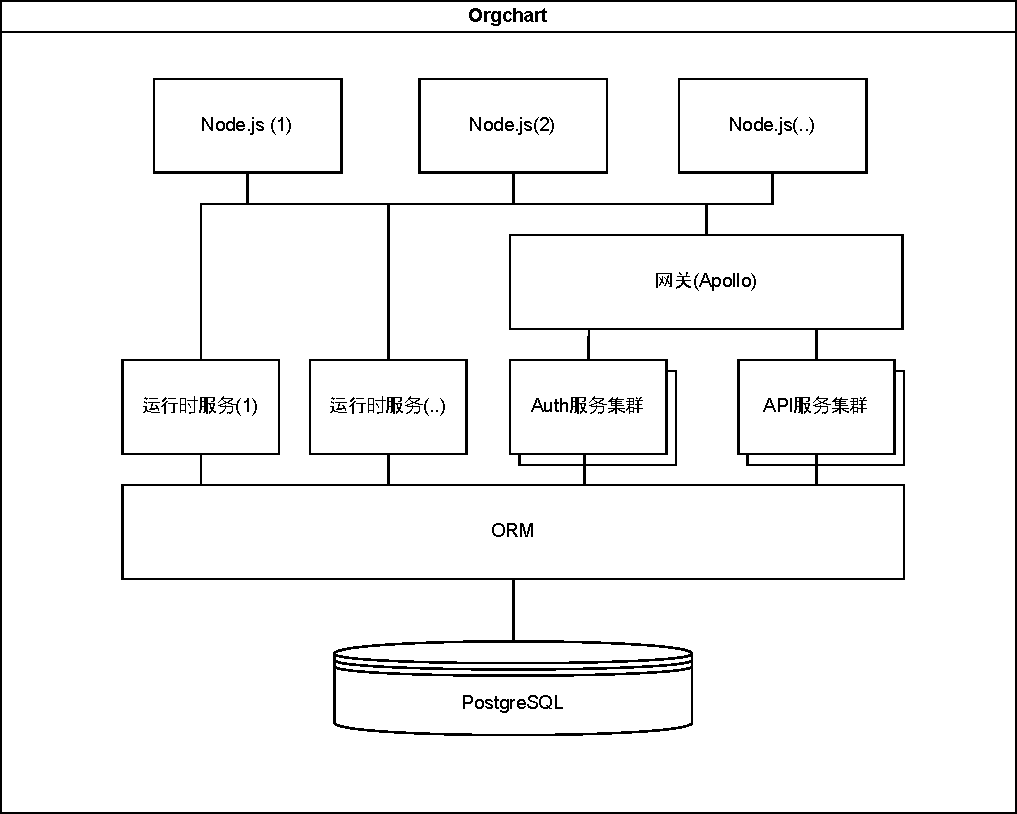
\includegraphics[width=0.95\textwidth]{figures/pdf/org.pdf}
    \caption{\label{org}系统架构组织图}
\end{figure}

本案符合非典型的web应用层次结构,分为表现层,接入层,业务逻辑层,数据访问层。
数据访问层采用名为 diesel 的 Rust crate 作为 ORM。
业务逻辑层分为Auth、API、Runtime等数个服务,每个服务都是独立的应用,可以横向扩展组成集群。
接入层使用 Apollo 作为 GraphQL 的网关,向外暴露所有的服务接口,还可以进行流量控制,但为了
支持运行时(Runtime)服务的“热插拔”,运行时服务并不会使用网关。
表现层使用 Node.js 作为 Web 的运行时,使用 React 作为 GUI 框架。
表现层和接入层、业务逻辑层使用 GraphQL 实现 Schema,使用 HTTP 和 WebSocket 协议通信,
GraphQL 是 Facebook开发的查询语言框架,其拥有不俗性能的同时解决很多RUSTful api的问题。\cite{hartig2018semantics}
同时GraphQL和React同为Facebook开发,因而十分适合在React环境中使用GraphQL\cite{taelman2018graphql}。

本案使用 actix-web 作为web服务端。WebSocket是一种网络传输协议,可在单个TCP连接上进行全双工通信,位于OSI模型的应用层。
WebSocket协议在2011年由IETF标准化为RFC 6455\cite{fette2011websocket},
后由RFC 7936补充规范。Web IDL中的WebSocket API由W3C标准化。

\subsection{生命周期与任务调度}
本案的元素围绕实例(instance)构成,一个典型的练习实例生命周期由以下几部分组成:
1)创建车站;
2)用户创建练习实例;
3)初始化实例;
4)访问实例;
5)结束实例。

其中,创建车站就需要用到后文提到的车站描述文件,车站被创建后将存入数据库中。创建好车站后,就可以创建
这个车站的实例。实例是uroj的最终端功能,是用户与联锁逻辑交互的直接对象,也是uroj的业务核心。
一个用户的一次练习就是一个实例,一个用户的一次考试也是一个实例。

本案支持预约或称定时开始的实例,在开始之前若用户尝试在executor
初始化一个实例,就会报错。在GUI上,在开始时间之前,不渲染开始按钮,和后端的时间约束形成两层约束。
实例创建后同样也会被记录在数据库中,当时间到后用户就可以在创建实例时指定的executor上
初始化实例 -- executor从数据库中读入instance,并运行。
实例初始化后用户就可以在该实例中进行进路车辆的各种操作。
最后实例会被结束。

在uroj的架构中,runtime服务(exexutor提供运行时服务,后文也称为“执行器”)的作用是实例运行的容器。其提供了
实例运行所需要的环境(如联锁逻辑、车站拓扑关系分析等)一个容器可以同时让多个
实例在其中运行。因此得名运行时或执行器。正如上表所示,一个车站可以创造无限个实例,
这也是本设计通用性的一大体现。

一个典型的考试实例生命周期由以下几步构成
1)创建车站;
2)创建考题、考试;
3)批量创建实例;
4)初始化实例;
5)访问实例;
6)结束实例。

和练习实例不同之处在于,一场考试是有考题的。同一场考试中无论考试有多少,考题
都是相同的。通过班级结构,可以在配置考试实例时指定受验班级,系统自动为
班级所有的学生创建配置信息完全相同(即开始时间、结束时间、考题、车站等等)的实例。

本案正是通过对于考题、车站等配置信息的最高效复用以实现通用性的。